\documentclass[a4paper,12pt]{article}

\usepackage[T2A]{fontenc}
\usepackage[utf8x]{inputenc}
\usepackage[russian,english]{babel}
\usepackage{graphicx}
\usepackage{color}
\usepackage{xcolor}
\usepackage{listings}
\usepackage{fancyhdr}
\usepackage{amsmath}
\usepackage{indentfirst} % включить отступ у первого абзаца

%%\usepackage[
%%		a4paper, includefoot,
%%		left=3cm, right=1cm, top=2cm, bottom=1.5cm,
%%		headsep=1cm, footskip=1cm
%%	]{geometry}

\title{Лабораторная работа №2}
\author{Кузнецов Д.Б.\and Вагин Д.А.}
\date{09/2010}
\pagestyle{empty}
\pagestyle{fancy}
\lhead{Лабораторная работа №2} %верхний колонтитул слева

\lstloadlanguages{c++,c}
\lstset{
	language=c,inputencoding=utf8x,
	extendedchars=\true,captionpos=b,tabsize=4,
	frame=lines,
	keywordstyle=\color{blue},commentstyle=\color{green},stringstyle=\color{red},
	breaklines=true,showstringspaces=false,basicstyle=\footnotesize
}

\begin{document}

\paragraph{Сравнение циклов и рекурсии}
\subparagraph{Цели}
\begin{itemize}
	\item Оценить недостатки процедурного программирования
	\item Научиться строить рекурсивные алгоритмы
\end{itemize}

\paragraph{Порядок выполнения}
\begin{enumerate}
	\item Написать программу по заданию с использованием цикла
	\item Провести трассировку программы
	\item Составить рекурсивную функцию для решения выданного задания
	\item Реализовать составленную рекурсивную функцию на языке программирования
	\item Написать отчет
\end{enumerate}

\subparagraph{Рекомендации по выполнению}
\begin{itemize}
	\item Массивы фиксированной длины
	\item Трассировка отключается макросом
	\item Данные задаются внутри исходного кода
\end{itemize}

\subparagraph{Состав отчета}
\begin{itemize}
	\item Титульный лист (фамилия, группа, номер варианта, наименование работы, задание)
	\item Текст рекурсивной функции
	\item Текст итеративной функции
	\item Результаты выполнения
\end{itemize}

\paragraph{Варианты заданий}
\begin{enumerate}
	\item Напишите программу печатающую $n$-ое число Фибоначчи.
	\item Напишите программу вычисляющую факториал натурального числа.
	\item Напишите программу проверяющую является ли введённое число простым.
	\item Напишите программу сортировки массива.
	\item Напишите программу поиска максимального элемента массива.
	\item Напишите программу возводящую одно натуральное число в степень другого, без использования функции возведения в степень.
	\item Напишите программу генерации всех правильных скобочных структур длины $2n$. Например для $n=3$ таких структур может быть 5: ()()(), (())(), ()(()), ((())), (()()).
	\item Имеется три стержня А, В, С. На стержень А нанизано $n$ дисков радиуса $1, 2,..., n$ таким образом, что диск радиуса $i$ является $i$-м сверху. Требуется переместить все диски на стержень В, сохраняя их порядок расположения (диск с большим радиусом находится ниже). За один раз можно перемещать только один диск с любого стержня на любой другой стержень. При этом должно выполняться следующее условие: на каждом стержне ни в какой момент времени никакой диск не может находиться выше диска с меньшим радиусом. 
	\item Заданы три числа: a, b, c. Необходимо выяснить, можно ли так переставить цифры в числах a и b, чтобы в сумме получилось c.
	\item Задан набор слов. Построить из них любую цепочку таким образом, чтобы символ в конце слова совпадал с символом в начале следующего.
	\item На рисунке показан пример треугольника из чисел. Написать программу, вычисляющую наибольшую сумму чисел, через которые проходит путь, начинающийся на вершине и заканчивающийся где-то на основании. 	
%		\begin{figure}
			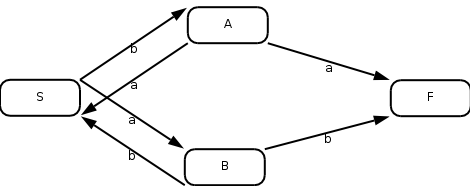
\includegraphics[scale=1.00]{images/image1.jpg}
%%			\label{fig:1}
%%		\end{figure}
		
\end{enumerate}

\paragraph{Пример}
\subparagraph{Задание}
Напишите программу проверяющую является ли введённое число факториалом какого либо числа.
\subparagraph{Итеративное решение}
Возьмём математическое определение факториала:
\begin{equation}
n! = 1\cdot 2\cdot\ldots\cdot n =\prod_{i=1}^n i
\end{equation}
Получается что факториал числа $n$ должен делиться нацело на все натуральные числа до $n$ включая $n$. Напишем программу рализующую такую проверку:

\begin{lstlisting}[language=c,{caption=итеративная программа}]
#include <stdio.h>

int check_factorial_iterate(int number){
	if(number < 0) 
		return 0;
	if(number == 0) 
		return 1;
	int i = 1;
	int n = 1;
	for(;n<number;n*=i,i++){
		
		if(number%i != 0)
			return 0;
	}
	return 1;
}

int main(){
	if(check_factorial_iterate(362880))
		printf("%s","yes");
	else
		printf("%s","no");
	return 0;
}
\end{lstlisting}

\subparagraph{Рекурсивное решение}
Возьмём рекурсивное определение факториала:
\begin{equation}
n!= \begin{cases}
1 & n = 0,\\
n \cdot (n-1)! & n > 0.
\end{cases}
\end{equation}

\begin{lstlisting}[language=c,{caption=рекурсивная программа}]
#include <stdio.h>

int check_factorial_recursive(int number, int i){
	if(number < 0) 
		return 0;	
	if(number == 0)
		return 1;

	if(number == 1)
		return 1;
	
	if( number%i != 0)
		return 0;
	else		
		return check_factorial_recursive(number/i,i+1);
	
}

int main(){
	int number = 362881;

	if(check_factorial_recursive(number,1))
		printf("%s\n","yes");
	else
		printf("%s\n","no");

	return 0;
}
\end{lstlisting}

\end{document}
